\section{Extended Reality}
\label{sec:background-intro}

\gls{XR} is an umbrella term encompassing all the possible combinations of real and virtual environments included in the spectrum of the \emph{Reality-Virtuality Continuum} (see \autoref{fig:virtuality-continuum}), introduced by Paul Milgram and Fumio Kishino in 1994 \cite{milgram_taxonomy_1994}.

\begin{figure}[h]
	\centering
	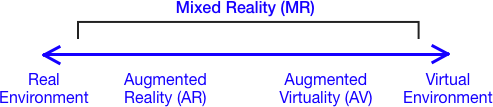
\includegraphics[width=7.5cm]{Background/virtuality-continuum.png}
	\caption{Milgram and Kishino's “Reality-Virtuality Continuum”}
	\label{fig:virtuality-continuum}
\end{figure}
In their work, the authors considered the real environment and \gls{VE}, also known as \gls{VR}, as two sides belonging to the same continuum, instead of two words in antitheses. Between them there exist other concepts with a variable quantity of real and VE such as \gls{AR} and AV. AR allows users to see the real world with virtual objects superimposed upon it, while with AV is the real world that augments the virtual environment. \gls{MR}, instead, has the peculiarity of mixing these two concepts, creating experiences in which physical and virtual objects co-exist and interact in real time with the user.

Some more emphasis on AR is put by Ronald Azuma \cite{azuma1997survey}, where the author defined three academic criteria for AR: it \textit{“combines the real and virtual”}, it is \textit{“interactive in real time”} and it is \textit{“registered in three dimensions”}. Later, Azuma et al.~\cite{azuma2001recent}, added that AR's objective is to \textit{“enhance the user’s perception of and interaction with the real world”}.

From this introduction it is clear that the “X” of XR represents a variable for any of these existing combinations. We have Augmented Reality (X=A, AR), Mixed Reality (X=M, MR) and Virtual Reality (X=V, VR). XR not only covers these environments but, as Honkanen \cite{honkanen_enhancing_2018} states, it is also the common term representing their immersive technologies and \textit{“human-device interaction aspects”}. Suh and Prophet \cite{suh_state_2018}, in their literature review on immersive technologies, describe XR as a means through which users' reality is extended as they feel placed within a simulation where real and simulated environments are indistinguishable \cite{kwok_covid-19_2020}.

A technical background of AR and VR is given by Egger et al.~\cite{egger_augmented_2020}. Generally, the main steps to produce AR experiences are twofold \cite{jenny_enhancing_2017}.
Content or landmarks indicating where AR is to be applied are detected in a first step. Subsequently, virtual objects are added above the camera feed based on the previously detected references \cite{parker_jr_augmented_2014}. Through the visors, devices equipped with a camera that captures the frames, it enables to see the AR information automatically i.e. without manual activation. In order to enable the device to recognize the real environment, the position of the user and what they are looking at, tracking must take place.Through the use of markers (\emph{marker-based} tracking), two-dimensional printed objects, objects in the real world are taken as landmarks. These identifiable elements can be scanned, so that the application software can interpret them and place the augmented objects or obtain information without using the geolocation. \emph{Marker-less} tracking) allows the use of sensors, such as accelerometer, cameras, GPS, to create anchor points based on recognisable features of the surrounding environment. \cite{egger_augmented_2020}.
Orthogonally to the tracking system used, another dimension to consider is the way we can experience AR:
\begin{enumerate}
	\item \glspl{HMD}, or “see-through AR glasses”, are a wearable device that work as normal glasses and contemporaneously have a small projector on the lenses to augment the real world with additional contents. The real environment is captured by the users by freely moving around it.
	\item Handheld devices equipped with all the components needed to record the real world and track its objects, e.g. camera, accelerometer and GPS. Most smartphones are equipped with these built-in instruments making AR widely used.
	\item Other forms of displays that do not belong to the Mobile AR (MAR) category (i.e. the two categories described above). An example of these displays are the AR mirrors often placed in open spaces that \textit{“do not require users to depend on any kind of device or application to experience AR”}.
\end{enumerate} 
VR, on the other hand, renders a totally VE that can be navigatd and interacted by the users, which one or more of their five senses are simulated in real-time \cite{guttentag_virtual_2020}. The author's study also defines two characteristics of VR: the ability to provide a physical immersion and a physical presence, making participants behave as in a real-life situation.
The VE, as explained by Egger et al., can represent either a computer-generated world or a 360$^{\circ}$ real-captured video or image.

Beck et al.~\cite{beck_virtual_2019} classify VR systems (VRs) distinguishing between non-, semi- and fully immersive VRs. The first term classifies desktop solutions allowing to navigate 360$^{\circ}$ videos and images in a classical PC interaction through mouse and keyboard. They are the simplest and most used form of VR, in platforms like YouTube and Facebook 360$^{\circ}$ Video. Semi-immersive systems have been used in the past years by projecting screens onto the walls and floor of a room and complementing the setting with spatial sounds, allowing a multi-user experience.
Fully immersive VRs, instead, require users to wear a \gls{HMD} that supports head tracking and other interactions through controllers or wearable devices, with the resulting feeling of a complete embodiment in the Virtual Environment.

Jung and Jeong \cite{jung_classification_2020} provide a further classification of VR devices according to the physical connectivity, tracking system and user behavior. Based on the physical connectivity there exist 4 categories that classify a VR device:
\begin{itemize}
    \item PC-tethered VR, Console-tethered VR: a VR headset connected to a desktop computer and a video game console that render the VE;
    \item Standalone VR: it is simply made by an untethered headset;
    \item Smartphone VR: a system made using a smartphone to render the graphics and a headset with lenses to recreate the VR effect.
\end{itemize}


In terms of tracking systems two technologies are used to track user's motion, the head tracking and position tracking: the latter uses the internal sensors of the headset (e.g. gyroscope, accelerometer and magnetometer), the former can be again divided into inside-out position tracking, which uses the camera on the headset to determine the movement, and outside-in position tracking that relies on external devices.
For what concerns user behavior categorization, VRs are divided into stationary VR, desktop-scale VR, room-scale VR and mobility VR. A VR device that does not have a position tracking feature can only be used in a stationary way, belonging to the stationary VR category; the desktop-scale VR and room-scale VR are opposites and refer to, respectively, systems with a restricted position tracking coverage and systems with a wider one. With a mobility VR device the user does not have space constraints and can, therefore, use it without spatial restrictions given its untethered nature and stand-alone position tracking component.